\section{Implementation}

\subsection{Systems Architecture}

\begin{figure}[H]
	\centering
	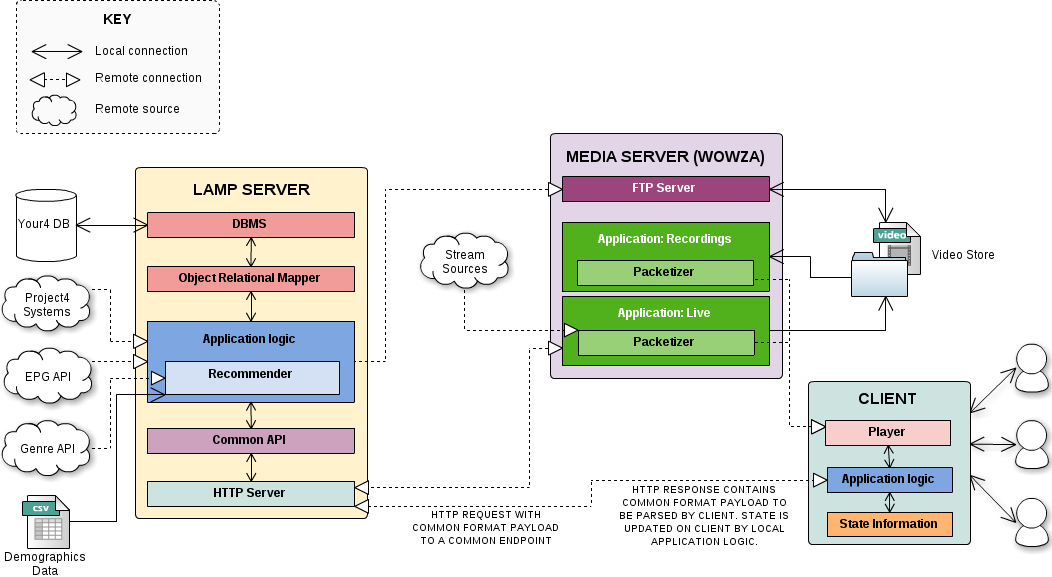
\includegraphics[scale=0.4]{images/your4-architecture.png}
	\caption{Overview of Your4 architecture}
	\label{your4-architecture}
\end{figure}

Figure~\ref{your4-architecture} shows the overall architecture of the Your4 system. The system is split into three distinct parts:

\begin{description}
	\item[Client] The client (expected to be Mobile Safari for iPad running on top of iOS 5+) is responsible for for interfacing with the LAMP server to retrieve the users' personalised playlist. With this playlist, the player in the client can then request the appropriate media from the media server.
	\item[LAMP server] The LAMP ()
\end{description}

\subsubsection{Client}
\subsubsection{LAMP Server}
\paragraph{REST Interface}
\paragraph{Recommender}
\subsubsection{Media Server}



\subsection{Languages and Techniques}
As this project involved interacting with many different systems, a diverse range of programming languages were used.

\subsubsection{Client-side web interfaces}
\begin{enumerate}
\item \textit{HTML}
\item \textit{CSS}
\item \textit{JavaScript}
\end{enumerate}

\subsubsection{Server-side and data-layer}
\begin{enumerate}
\item \textit{PHP}
\item \textit{Python}
\end{enumerate}

Communication between server and client is done through a REST interface.

Datebase is MySQL.

\subsubsection{Streaming server}
\begin{enumerate}
\item \textit{Java} to interface with the Wowza streaming server
\item \textit{Python} to interpret to GPI[?] pulse in order to establish when breaks in live programmes are
\end{enumerate}

\subsection{Libraries and Frameworks}

\subsection{Detailed Architecture}

\subsubsection{Database structure}

\subsubsection{Programme recommendation}

\subsubsection{Advert selection}

\subsubsection{REST services}

\subsubsection{Playback}
Plays HLS streams in HTML5 Video tag, or RTMP stream in Flash Video.

The player must be capable of displaying two types of media: \textit{video} (for programmes and video adverts) and \textit{stills} (for adverts which consist of just one picture). Additionally, some adverts may have an overlay, which consists of some HTML specified by the advertiser. A challenge here is hiding the buffering of videos or loading of images. A solution is to hide any media until it has loaded. Layers:
\begin{enumerate}
\item \textit{Black layer}: used to hide any loading media
\item \textit{Overlay layer}: an iFrame which will display the HTML that the advertiser has specified for the overlay
\item \textit{Still layer}: an image that will display any still adverts
\item \textit{Video layer}: the video component to show the video
\end{enumerate}

\subsubsection{Data visualisation}


\subsection{Code Statistics}
Lines of code in JS, PHP, Java, Python, HTML, CSS etc

\subsection{System walkthrough}
\begin{figure}[th]
	\centering
	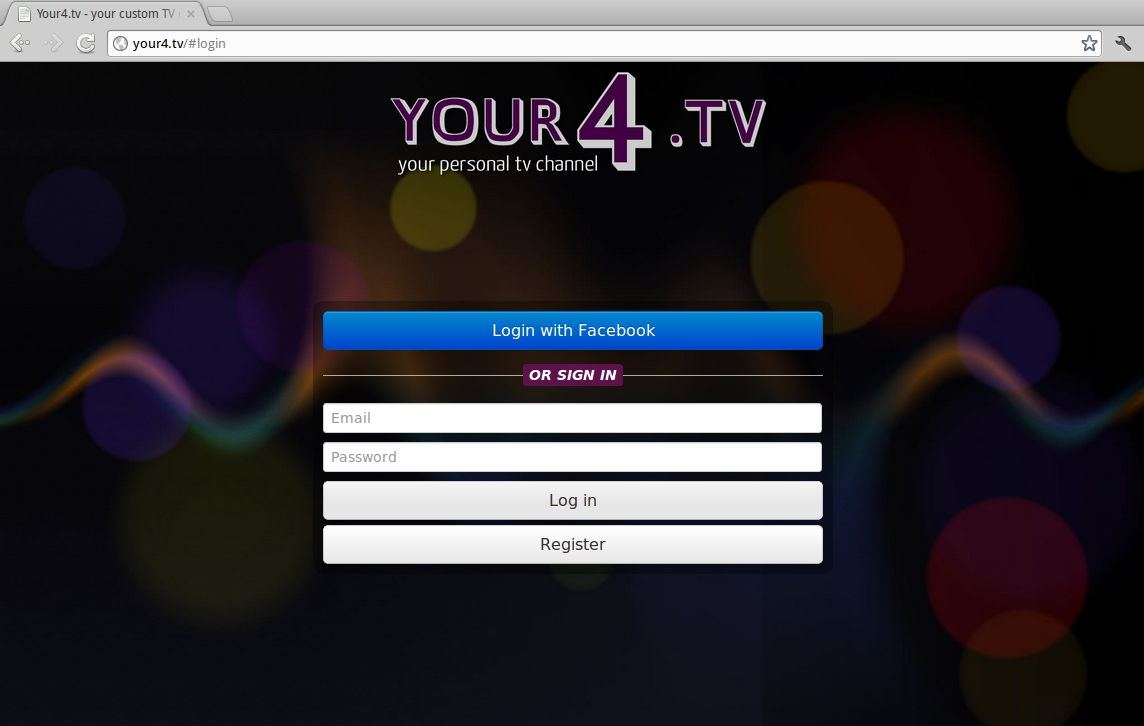
\includegraphics[width=\textwidth]{images/screenshots/your4-login.png}
	\caption{Log in}
	\label{fig:your4-login}
\end{figure}
\begin{figure}[th]
	\centering
	
\includegraphics[width=\textwidth]{images/screenshots/your4-tap-to-start.png}
	\caption{Log in}
	\label{fig:your4-tap-to-start}
\end{figure}
\begin{figure}[th]
	\centering
	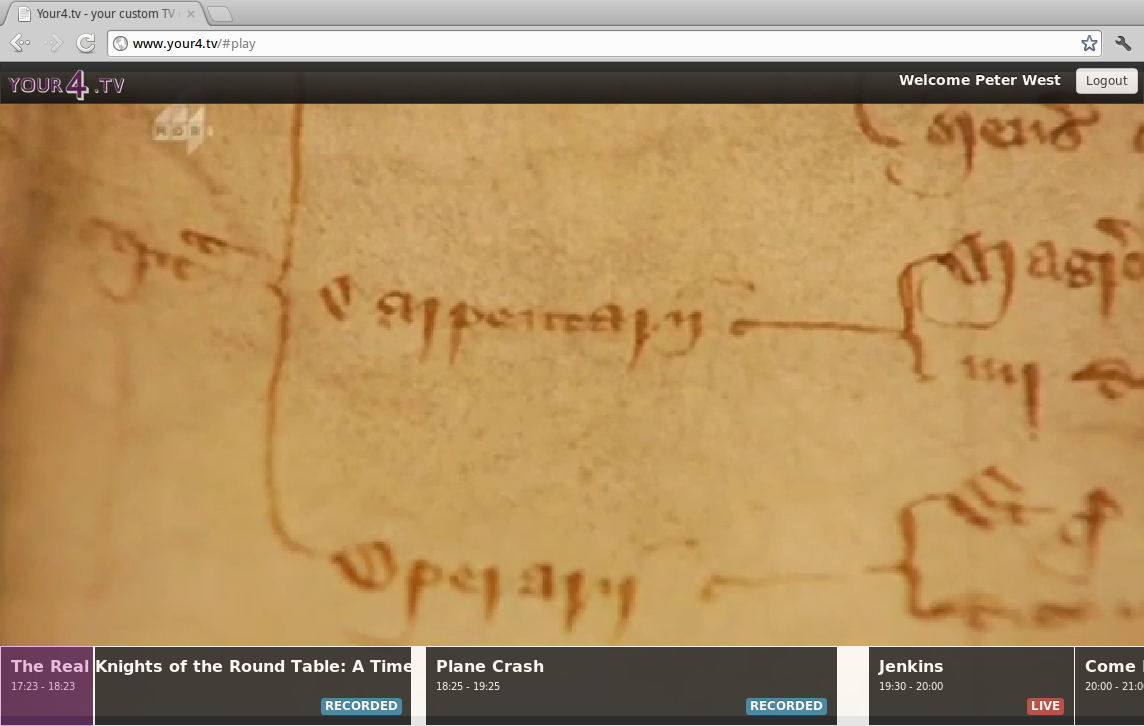
\includegraphics[width=\textwidth]{images/screenshots/your4-play.png}
	\caption{Log in}
	\label{fig:your4-play}
\end{figure}

\begin{figure}[th]
	\centering
	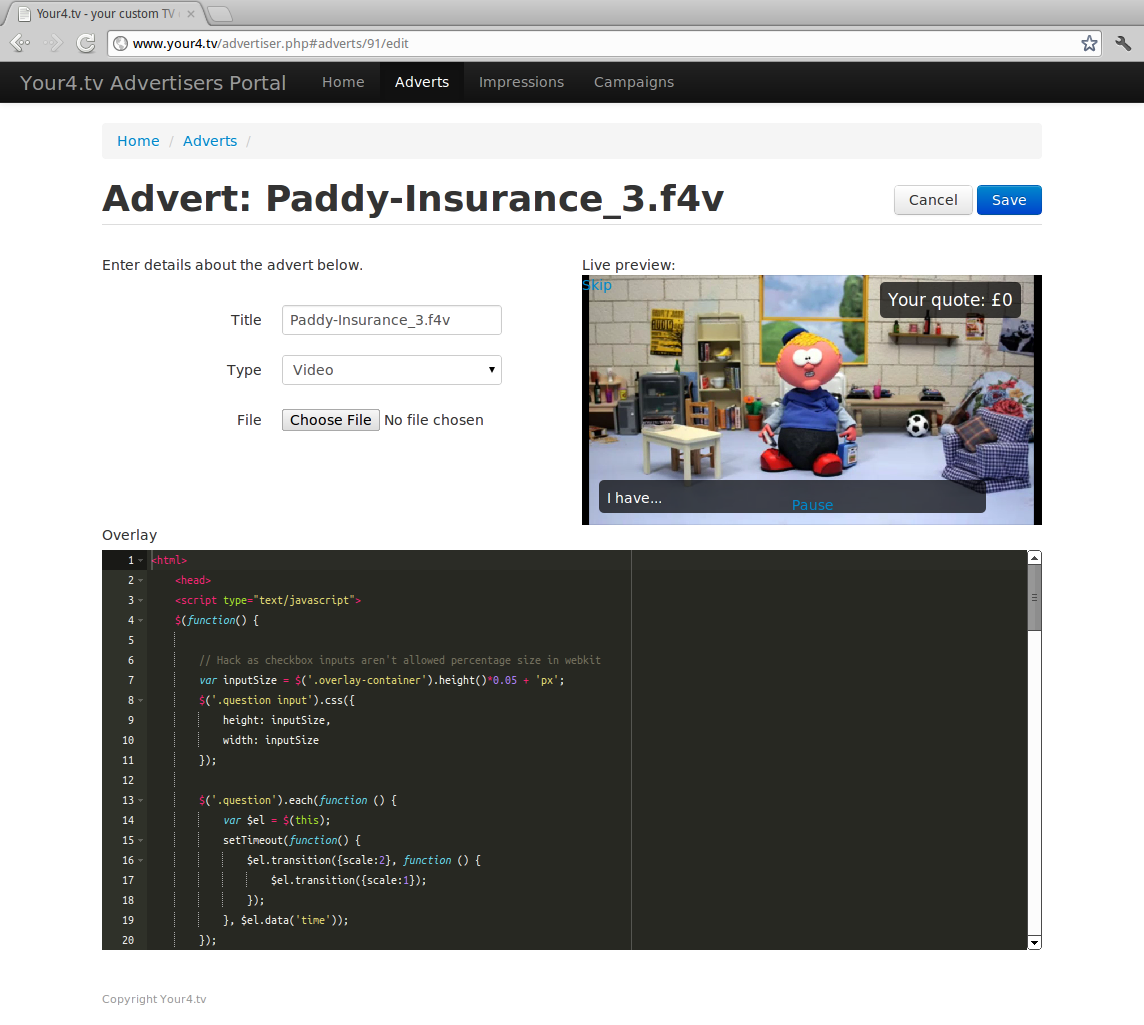
\includegraphics[width=\textwidth]{images/screenshots/advertiser-advert-edit.png}
	\caption{Log in}
	\label{fig:advertiser-advert-edit}
\end{figure}
\begin{figure}[th]
	\centering
	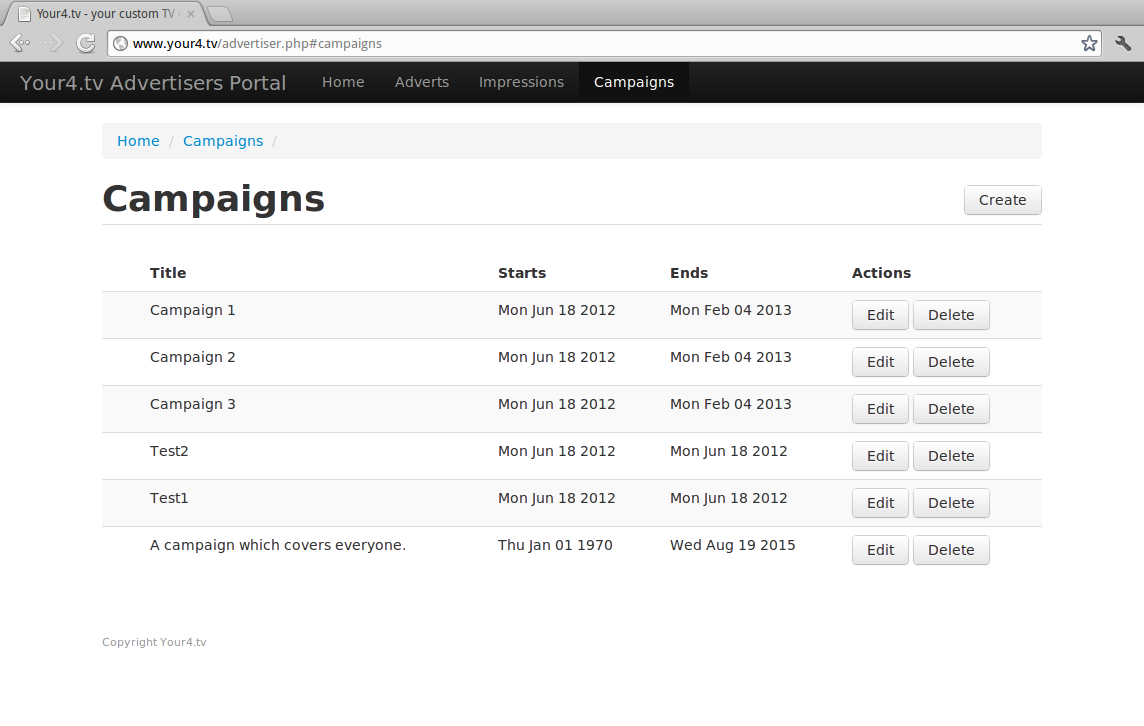
\includegraphics[width=\textwidth]{images/screenshots/advertiser-campaigns.png}
	\caption{Log in}
	\label{fig:advertiser-campaigns}
\end{figure}
\begin{figure}[th]
	\centering
	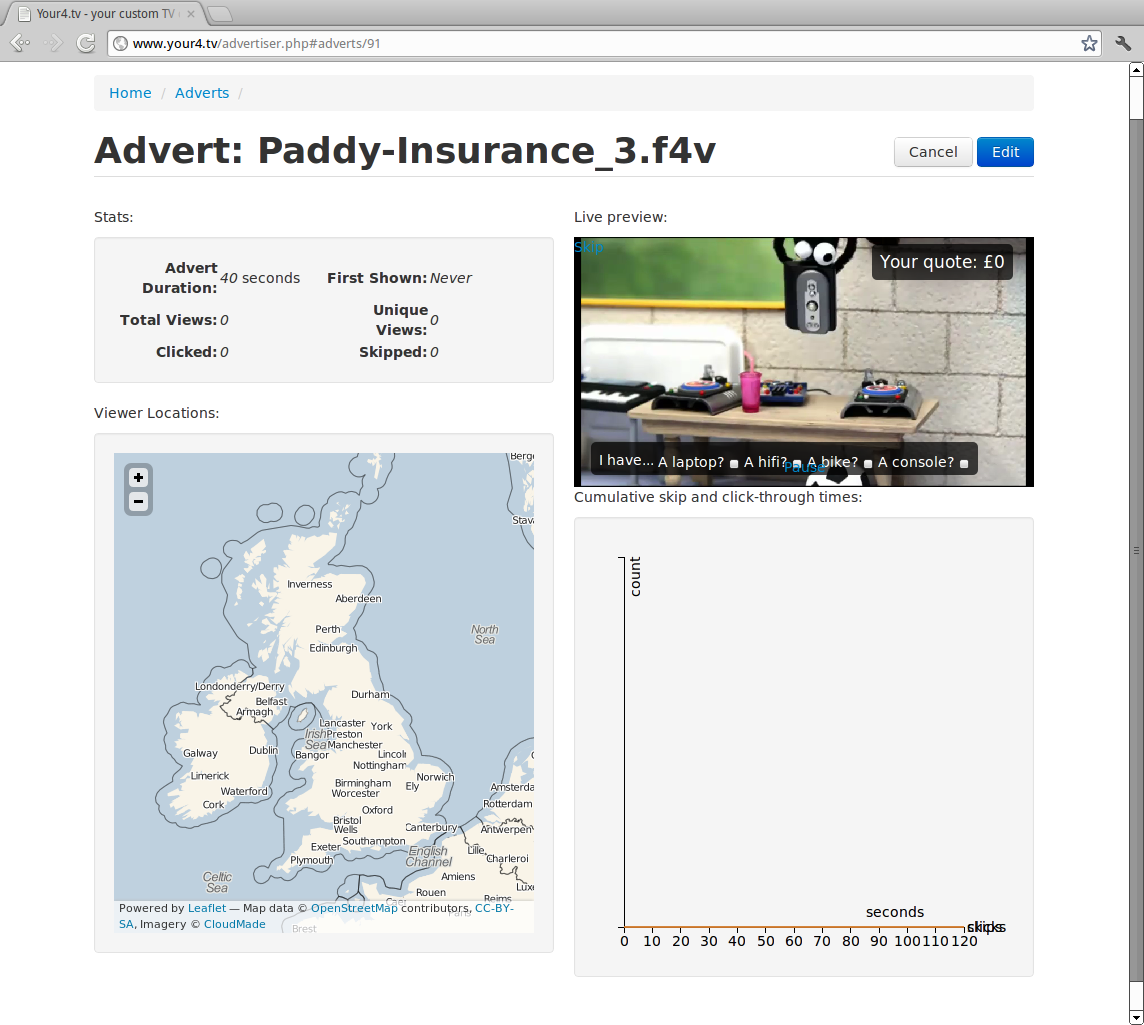
\includegraphics[width=\textwidth]{images/screenshots/advertiser-advert.png}
	\caption{Log in}
	\label{fig:advertiser-advert}
\end{figure}
\begin{figure}[th]
	\centering
	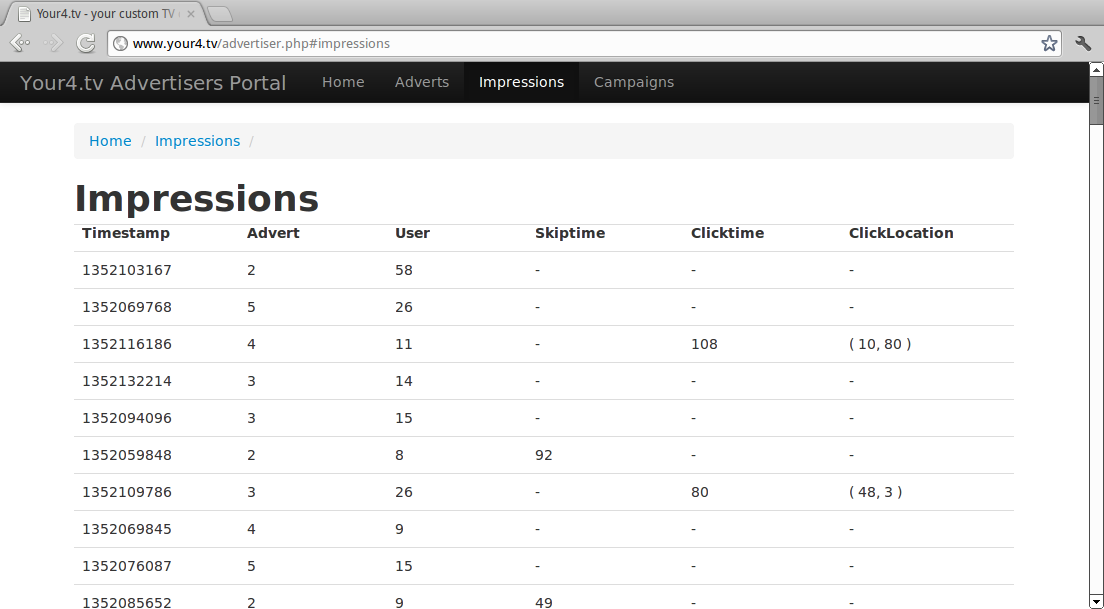
\includegraphics[width=\textwidth]{images/screenshots/advertiser-impressions.png}
	\caption{Log in}
	\label{fig:advertiser-impressions}
\end{figure}
\begin{figure}[th]
	\centering
	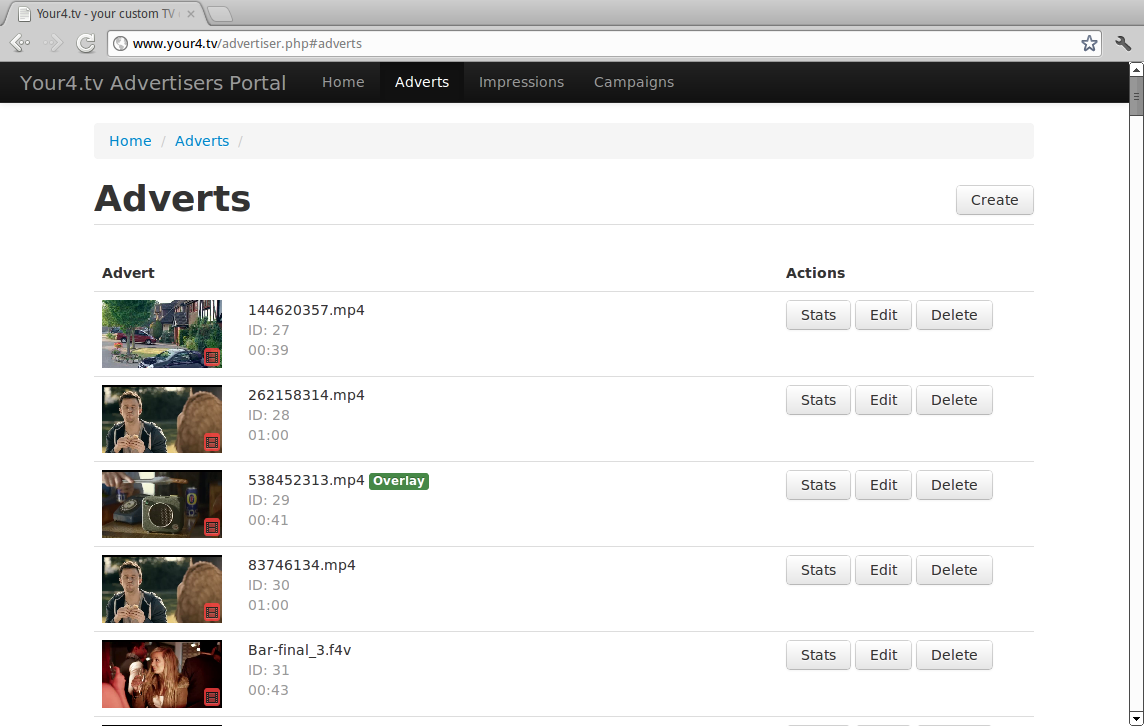
\includegraphics[width=\textwidth]{images/screenshots/advertiser-adverts.png}
	\caption{Log in}
	\label{fig:advertiser-adverts}
\end{figure}
\begin{figure}[th]
	\centering
	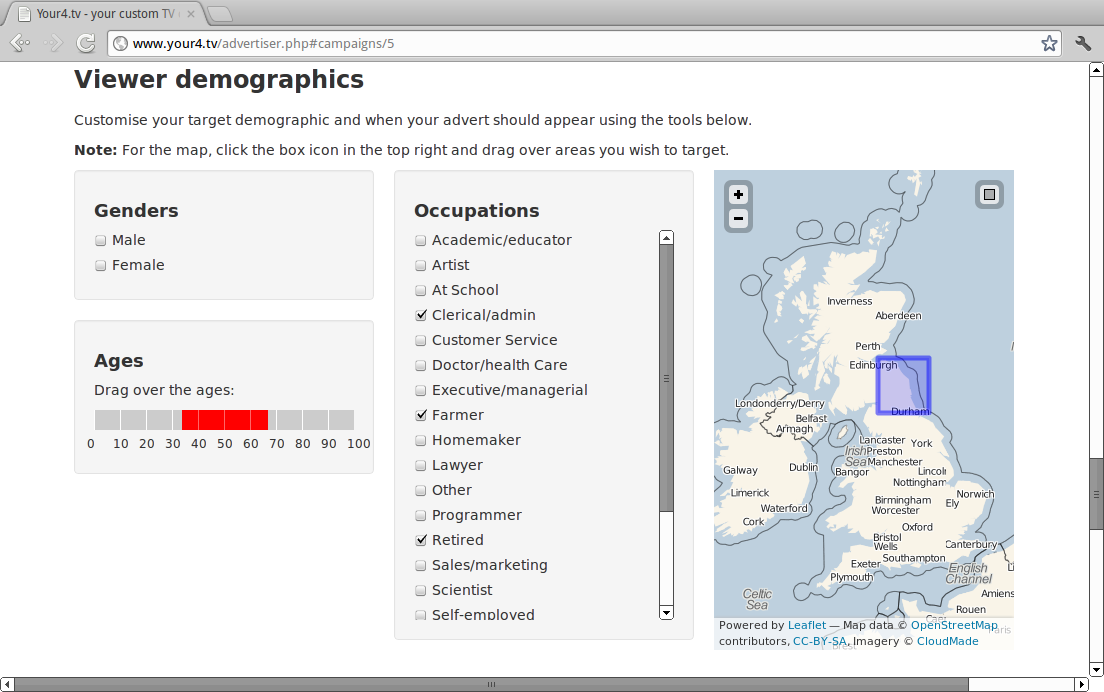
\includegraphics[width=\textwidth]{images/screenshots/advertiser-campaign-demographics.png}
	\caption{Log in}
	\label{fig:advertiser-campaign-demographics}
\end{figure}
\begin{figure}[th]
	\centering
	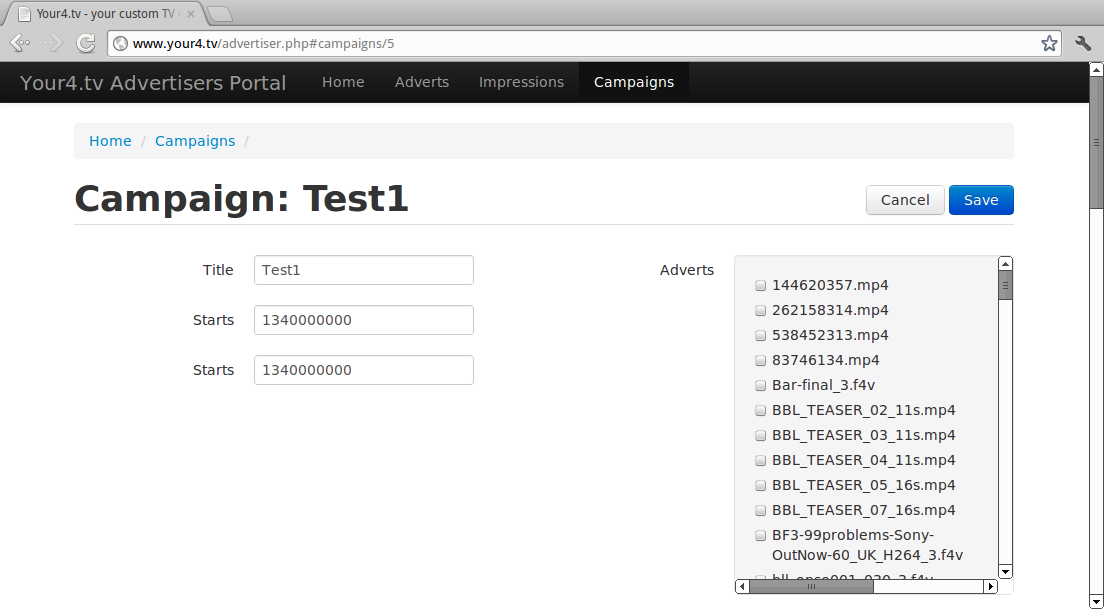
\includegraphics[width=\textwidth]{images/screenshots/advertiser-campaign.png}
	\caption{Log in}
	\label{fig:advertiser-campaign}
\end{figure}
\begin{figure}[th]
	\centering
	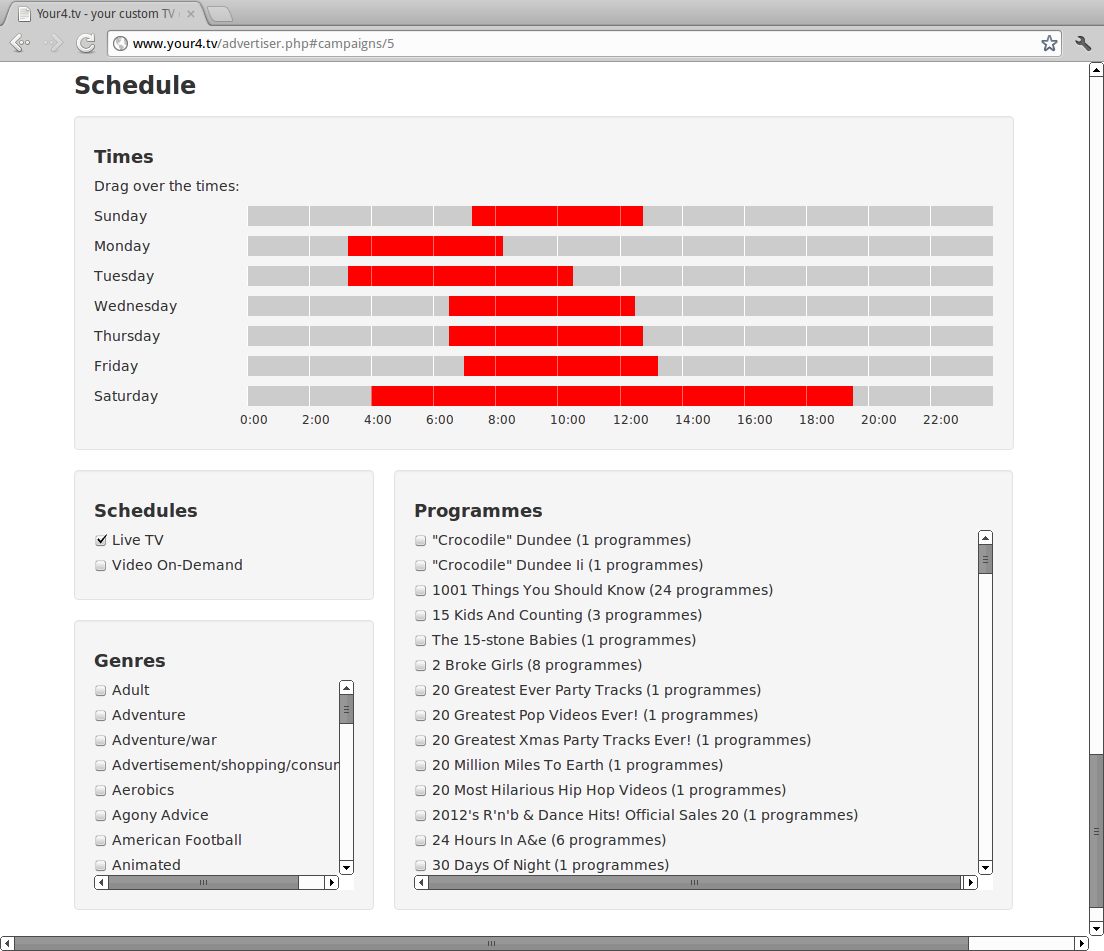
\includegraphics[width=\textwidth]{images/screenshots/advertiser-campaign-schedule.png}
	\caption{Log in}
	\label{fig:advertiser-campaign-schedule}
\end{figure}